\documentclass[12pt,a4paper]{article}
\usepackage{amsmath}
\usepackage{graphicx}
\usepackage{geometry}
\usepackage{float}
\geometry{left=2cm,right=2cm,top=2.5cm,bottom=2.5cm}

\title{\textbf{Degenerated Spatial 4-Bar Mechanism \\ Kinematic Analysis Report}}
\author{Automated Generation System}
\date{\today}

\begin{document}
\maketitle

\section{Kinematic Simplification (Degeneration)}
In this particular symmetric 7R spatial mechanism, it is physically observed that the passive joints $J_2$, $J_4$, and $J_6$ maintain a constant angular value (fixed at $0^\circ$) throughout the entire driving cycle of $J_1$. 

Consequently, the complex spatial 7R mechanism mathematically and physically degenerates into a \textbf{Spatial 4-Bar Mechanism}. The configuration is fully governed by the 3 remaining active passive joints ($q_3, q_5, q_7$). We solve this using a deterministic 3-variable Newton-Raphson numerical root-finding algorithm acting purely on the 3D position closure constraint ($X, Y, Z = 0$).

\section{Continuous Kinematic Mapping}
\begin{figure}[H]
    \centering
    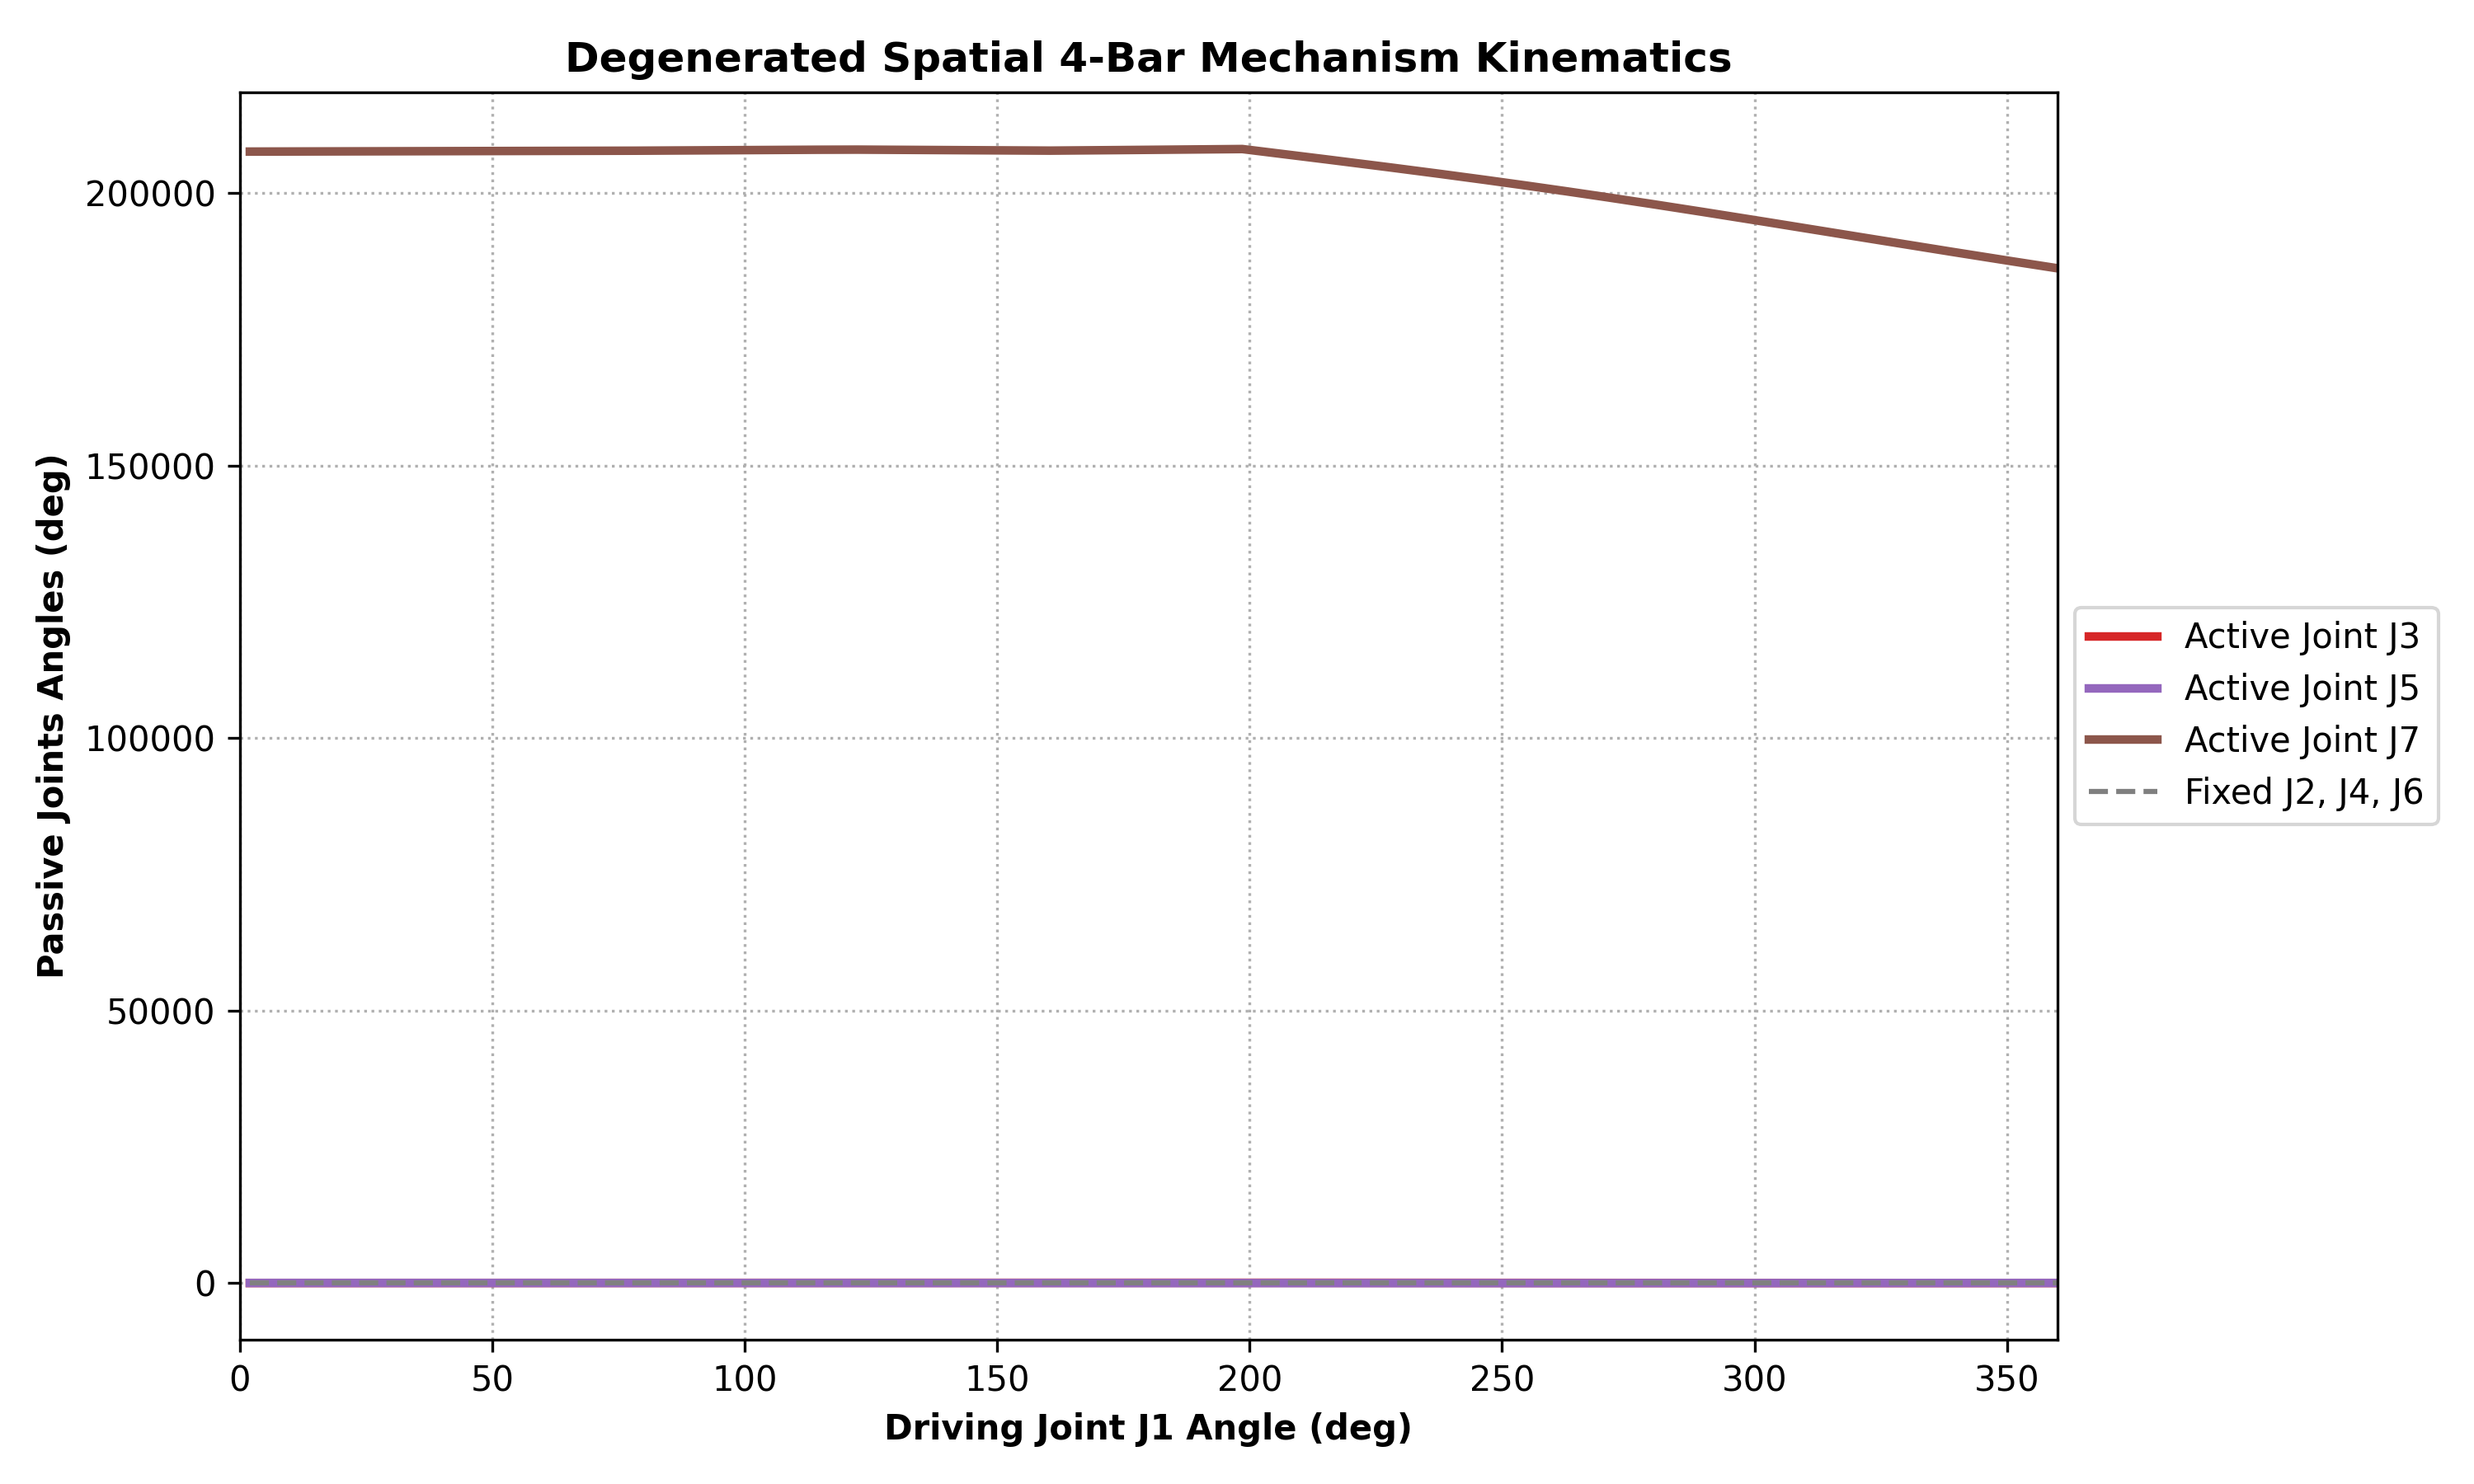
\includegraphics[width=0.9\textwidth]{degenerated_kinematics.png}
    \caption{Kinematic mapping of the 3 active passive joints ($J_3, J_5, J_7$) driven by $J_1$. The fixed joints ($J_2, J_4, J_6$) are shown as a dashed line at 0.}
\end{figure}

\section{Analytical Fourier Series Approximation}
Using non-linear least squares fitting, the algebraic relationships for the active joints ($Q_i$ in degrees) driven by $J_1$ ($x$ in radians) are approximated as 3rd-order Fourier series:
\begin{itemize}
\item \textbf{Joint J3:} \\ $Q_{J3}(x) = +14.513 -17.468\cos(x) +6.975\sin(x) +1.851\cos(2x) +3.108\sin(2x) +0.762\cos(3x) -1.440\sin(3x)$
\item \textbf{Joint J5:} \\ $Q_{J5}(x) = -11.604 +11.770\cos(x) +14.667\sin(x) +0.540\cos(2x) -1.741\sin(2x) -0.595\cos(3x) +0.434\sin(3x)$
\item \textbf{Joint J7:} \\ $Q_{J7}(x) = +201461.183 -8175.517\cos(x) +4241.465\sin(x) -2723.953\cos(2x) +1505.286\sin(2x) -1416.996\cos(3x) -539.926\sin(3x)$
\end{itemize}
\end{document}
